\documentclass[main.tex]{subfiles}

\begin{document}


\chapter{Introduction}

\setlength{\epigraphwidth}{0.75\textwidth}
\renewcommand{\textflush}{flushepinormal}
\epigraph{The major challenge for language documentation in the next decade or two is what could be called the transcription challenge. This is a multilayered challenge that goes far beyond the practical challenge of speeding up the transcription process. [...] Despite its centrality to language documentation, transcription remains critically undertheorized and understudied. Further progress in language documentation, and ultimately also its overall success, crucially depends on further investigating and understanding the transcription process, broadly conceived.}%
         {\justifying\fullcite{himmelmann2018meeting}}

Language documentation is typically considered a sub-field of linguistics and its purpose is ``to provide a comprehensive record of the linguistic practices characteristic of a given speech community'' \parencite[][p.~166]{himmelmann1998documentary}.~Many aspects of its practice, however, require continual integration of developments beyond linguistics.~As the target languages are often spoken by minoritised Indigenous communities, it is necessary to proactively consider evolving norms regarding fair and ethical collaboration \parencite{holton2022indigenous}.~Concurrently, data protocols must not only continually integrate these norms but also technological advancements that more effectively enable the creation, processing, storage, and distribution of recorded materials \parencite{berez2023recent}.~In both respective areas, there are ongoing developments that constitute paradigm shifts:~1) decolonising, community-centred approaches to working with Indigenous communities, and 2) speech and language processing systems powered by foundation models (FMs).~Integrating considerations from the former and leveraging advancements in the latter, I examine in this dissertation how these FM-powered systems can help create contextually-appropriate solutions to combat a major bottleneck in language documentation workflows --- the transcription of recorded materials.

\section{Language documentation and the transcription bottleneck}

It is generally recognised that there are about 7,000 languages spoken in the world today and that at least half of them may not exist by the end of the century \parencite{austin2011cambridge}.~Many of these languages are spoken by Indigenous and minoritised communities, who are under cultural, economic, and technological pressures to shift to using more dominant regional, national, or global languages.~For example, education may be conducted entirely in more widely-used regional or national languages and technological interfaces may only exist in a national or global language.~Such pressures can lead to language endangerment, as younger generations gradually adopt the more widely-used languages until there remain no living first-language or `L1' speakers, at which point a language may become `dormant'.

There are many ongoing revitalisation efforts to fight these pressures by encouraging the learning and active use of endangered languages, safeguard the knowledge of elder L1 speakers by recording them, as well as efforts to ‘awaken’ dormant ones based on archival recordings.~However, as recording speech is considerably easier than transcribing the recorded speech, many recording collections of these languages remain only partially transcribed, if at all \parencite{cox2019taking}.~Yet, raw audio data comprising untranscribed speech is difficult to index and search, limiting how efficiently content within the materials can be discovered and used (e.g. for creating language learning materials).~Indeed, the difficulty is so ubiquitous that it has been termed the ``transcription bottleneck'' \parencite[]{seifart2018language,foley2018building,cox2019taking} and the consequences of hard-to-access materials so dire that there are warnings against inadvertently creating ``data graveyards, i.e. large heaps of data with little or no use to anyone'' \parencite[][p. 4]{himmelmann2006language}.

There are several contributing factors that result in this bottleneck with respect to transcribing minoritised languages.~First, unlike major languages such as English, searchable high-quality transcriptions cannot simply be derived using a high-performance automatic speech recognition (ASR) system, whose development itself has conventionally required large quantities of transcribed speech.~Second, there is typically no option for large-scale crowd-sourcing of target language transcriptions as by definition of endangerment there may be very few speakers and only a subset of speakers may be literate in this language (i.e.~not the regional or national language of formal education).~Third, there may not be a standardised orthography for the target language, in which case a project-specific working orthography is often developed, resulting in transcriptions with both intra- and inter-transcriber variation, requiring additional time for review and corrections.~Finally, in some instances, there may also be an additional personnel bottleneck resulting from limitations on who can listen to and transcribe certain recordings (e.g.~of culturally-sensitive materials such as descriptions of ceremonial procedures).~Taken altogether, surveys of transcription time have reported typically requiring about 30 to 50 hours of work to transcribe one hour of recorded speech \parencite{durantin2017survey,michaud2014towards,zahrer2020towards}.

Reviewing a century of transcription practice within linguistics, \textcite{bird-2020-sparse} argues that several parts of the transcription bottleneck are a result of a description- and analysis-centred transcription practice, which he terms `contiguous' and suggests a more `sparse' approach.~He identifies three inefficient characteristics particular to orthodox transcription practice:~1) transcribing phones,~2) transcribing fully, and 3) transcribing first (before translating).~We review these characteristics using a Samoan utterance sourced from my Field Methods class recordings, illustrated above in in Figure \ref{fig:how-lift-boat-tf}.~Given my goal of grammatically analysing a language largely unknown to me, I am primarily interested in textually representing the form of the spoken utterance, leading to a primary focus on the phonetic form of the whole utterance [{\fontspec{LinLibertine.ttf}sasiʔielevailevaʔa}], with the translation secondary.~Using these annotations along with other data points, I can hypothesise what the various lexical and grammatical units are in Samoan and how they interact,~e.g. [sa]+[siʔi] P{\footnotesize{}ST}+lift `lifted'.

\begin{figure*}[t]
  \centering
  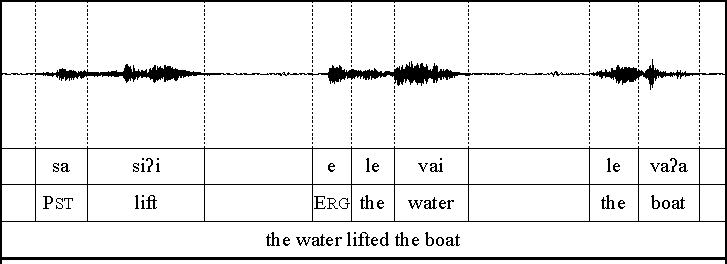
\includegraphics[width=0.75\linewidth]{figures/intro-conventional-transcription}
  \caption{A fully transcribed and translated Samoan utterance.}
\label{fig:how-lift-boat-tf}

  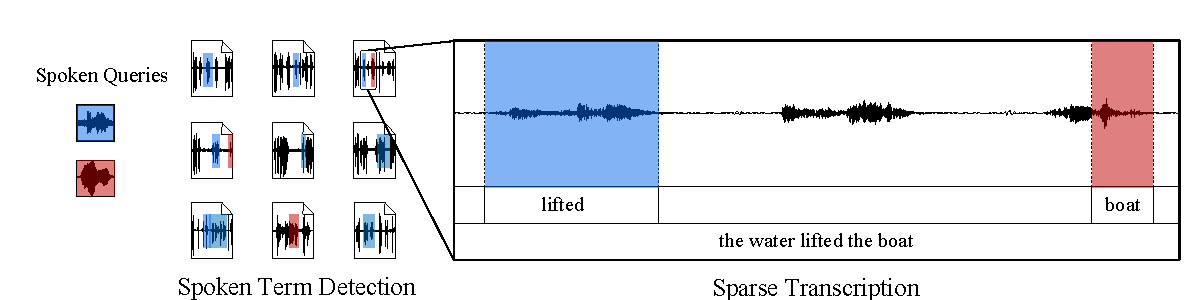
\includegraphics[width=1.0\linewidth]{figures/intro-sparse-transcription}
  \caption{A sparsely transcribed and translated Samoan corpus and utterance.}
  \label{fig:how-lift-boat-sparse}
\end{figure*}

% \begin{figure*}[b]
%   \centering

% \end{figure*}

\textcite{bird-2020-sparse} questions whether this conceptualisation of transcription effectively serves the many parties interested in working with untranscribed language documentation corpora, particularly those of unwritten, oral languages.~Intended as a supplementary approach, \textcite{bird-2020-sparse} proposes `sparse transcription' which does away with the three characteristics that contribute to the bottleneck in conventional transcription and, importantly, facilitates access to untranscribed language documentation corpora in ways that are more compatible with the skills of the speech communities.~As illustrated in Figure \ref{fig:how-lift-boat-sparse}, spoken term detection or `word spotting' is used to facilitate searches via spoken queries (i.e.~a voice-based alternative to text queries on transcriptions) and, upon confirmation of hits, speakers literate in the language of wider communication can also provide translations.~In this way, the confirmed locations of various queries along with their translations allow for the corpus to be collaboratively and iteratively indexed, albeit sparsely.~Additionally, this supplementary approach can help more effectively find regions of interest in the corpora to which conventional `full' transcription efforts can be directed. 

Following the proposal of the sparse transcription model by \textcite{bird-2020-sparse}, there have been several studies investigating its potential in various workflow configurations and documentation scenarios \parencite{leferrandEnablingInteractiveTranscription2020,le2021phone,le2022learning,lane2022finite,lane2021local}.~One area that has been identified for improvement is the robustness of the spoken term detection system, particularly for scenarios where the speaker of the query is different to the speakers in the corpus and when the audio of the corpus is relatively noisy.~We return to this discussion below in our review of foundational models for speech and subsequent investigation of whether these models help deliver more speaker-invariant and noise-robust spoken term detection systems.

Even without a robust spoken term detection system, it may nevertheless be possible to derive a searchable index for mixed-language documentation corpora where the target language being documented is inter-mixed with a more widely spoken language for metalinguistic questions and commentary.~As illustrated below in Figure \ref{fig:mixed}, the response by the Samoan speaker was preceded by my elicitation prompt in English:~\textit{How do you say ``the water lifted the boat''?}~As mentioned above, it is relatively straightforward to derive searchable high-quality transcriptions using a high-performance ASR system for major languages such as English.~As such, if foundation models can be used to isolate and transcribe the more widely used language, these searchable metalanguage transcriptions could provide approximate locations where certain target language words and topics are being discussed in mixed-language documentation corpora of this genre.

\begin{figure*}[t]
  \centering
  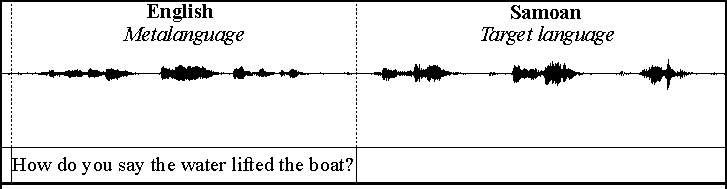
\includegraphics[width=0.85\linewidth]{figures/intro-mixed-corpus.pdf}
  \caption{Sparse transcription via automatic isolation and machine transcription of a more widely used metalanguage in a mixed-language corpus.}
  \label{fig:mixed}
\end{figure*}

Ultimately sparse transcription is intended as a way to ``accelerate [the work of] orthodox, contiguous transcription'' \parencite[p.~737]{bird-2020-sparse} while also facilitating immediate access to untranscribed speech corpora.~If, on one hand, sparse transcription can help efficiently gather the target language transcriptions and, on the other, foundation models can be used to substantially reduce the amount of target language transcriptions required to begin ASR system development, this combination could provide a pathway for creating ASR-assisted transcription workflows for minoritised languages.

\section{Foundation models for speech processing}

\end{document}